\documentclass[11pt,a4paper]{article}
\usepackage[margin=2.3cm]{geometry}
\usepackage{amsmath,amssymb}
\usepackage{booktabs,tabularx,array}
\usepackage{pgfplots}
\pgfplotsset{compat=1.18}
\usepackage[font=small,labelfont=bf]{caption}
\usepackage{enumitem}
\usepackage{hyperref}
\hypersetup{colorlinks=true,linkcolor=black,urlcolor=blue!60!black,citecolor=black}
\setlength{\parskip}{0.45em}
\setlength{\parindent}{0pt}
\setlist{itemsep=0.15em,topsep=0.3em}
\newcolumntype{L}{>{\raggedright\arraybackslash}X}

\title{\vspace{-1.2cm}\textbf{Shared Control of a BCI-Driven Wheelchair}\\[3pt]
\large Stage 1 Report: EEG Decoding and Baseline Characterisation}
\author{Pragyan Mohanty \quad|\quad Roll No.\ 24250 \quad|\quad Control Systems Project}
\date{Mid-Semester Submission, September 2026}

\begin{document}
\maketitle
\vspace{-0.6cm}

\begin{abstract}
\noindent A motor-imagery brain--computer interface (BCI) is an unreliable control
channel. It is often wrong, it responds late, and it updates slowly. This project
studies how control authority should be shared between a BCI user and an
autonomous navigator so that a wheelchair remains stable and safe. Stage~1
establishes the empirical basis for that study. A conventional CSP--LDA decoder
was trained and evaluated across recording sessions on BCI Competition~IV
Dataset~2a. Over nine subjects it reaches a mean accuracy of 0.443 against a
chance level of 0.25. Calibration reduces the expected calibration error from
0.196 to 0.096, and median decision latency ranges from 2 to 4\,s. These
parameters are now frozen and define the channel model for Stage~2.
\end{abstract}

\section{Problem Statement and Objective}

Motor-imagery BCIs decode imagined limb movements from scalp EEG and give people
with severe motor impairment a way to issue commands. As a control input,
however, the decoded signal is a degraded measurement of user intent. It has a
high error rate, a transport delay of several seconds, and an update rate limited
by the decoder's decision window. Closing a feedback loop directly through such a
channel compromises both stability and safety.

The objective is to design and analyse a shared-control law that allocates
authority between the user and an autonomous navigator, keeping the closed loop
stable under transport delay and safe under decoder error while preserving as
much user authority as possible. The work is divided into two stages. Stage~1
characterises the decoder from real data. Stage~2 designs and optimises the
control law around that characterisation. The order is deliberate: the
disturbance model used in Stage~2 must be measured, not assumed.

\section{Proposed Solution}

The actuator command is a convex combination of the decoded user command and the
autonomous command,
\begin{equation}
u(t) = \alpha(t)\,u_{\mathrm{BCI}}(t) + \bigl(1-\alpha(t)\bigr)\,u_{\mathrm{auto}}(t),
\qquad \alpha \in [0,1],
\end{equation}
with the authority adapted online from the decoder's calibrated confidence $c$
and a situational risk signal $r$,
\begin{equation}
\alpha = c\,(1-r).
\end{equation}
For fixed $\alpha$ and total loop delay $\tau$, one axis of the blended loop has
the characteristic equation
\begin{equation}
\Delta(s) = s^2 + d\,s + (1-\alpha)(K_1 + K_2 s) + \alpha\,(K_p + K_d s)\,e^{-\tau s} = 0,
\end{equation}
where $K_1, K_2$ are the LQR gains and $K_p, K_d$ the operator gains. The loop
is stable for any delay when $\alpha < \alpha^* = K_1/(K_1 + K_p)$.

\subsection*{Framework}
{\small\noindent
\begin{tabularx}{\textwidth}{@{}p{4.1cm}L@{}}
\toprule
\textbf{Concept} & \textbf{Role in the project} \\
\midrule
EEG decoding & Common Spatial Patterns and shrinkage LDA on the 8--30\,Hz band ($\mu$ and $\beta$ rhythms) \\
Probability calibration & Platt scaling; quality measured by expected calibration error (ECE). Supplies the confidence $c$ \\
Stochastic channel model & Two-state Markov error process (reliable/degraded) with measured latency and confusion structure \\
Plant dynamics & Unicycle wheelchair with first-order actuator lag; damped double integrator $\dot p = v,\ \dot v = u - d\,v$ for analysis \\
Operator model & Delayed PD controller, $u_h(t) = K_p\,e(t-\tau_h) - K_d\,v(t-\tau_h)$ \\
Optimal control & LQR, with gains from the algebraic Riccati equation \\
Obstacle avoidance & Dynamic Window Approach over the velocities reachable under actuator limits \\
Situational risk & Time-to-collision mapped to $r \in [0,1]$ and low-pass filtered \\
Authority conditioning & Schmitt-trigger hysteresis and slew-rate limiting on $\alpha$ \\
Time-delay stability & Substituting $s=j\omega$ removes $\tau$ from the magnitude condition, leaving a quadratic in $\omega^2$ and a closed-form delay margin $\tau_{\max}(\alpha)$ \\
Verification & Pad\'e (2,2) comparison, DDE simulation and bisection, the \texttt{control} package, and MATLAB \\
Statistics & Paired Monte-Carlo runs with subject-level bootstrap confidence intervals \\
\bottomrule
\end{tabularx}\par}

\section{Dataset}

The study uses BCI Competition~IV Dataset~2a (BNCI2014\_001), accessed through
MOABB and MNE-Python: nine subjects, 22 EEG channels at 250\,Hz, and four
imagined movements (left hand, right hand, feet, tongue), mapped to turn left,
turn right, forward and stop. Each subject was recorded in two sessions on
different days, with 288 balanced trials per session. The decoder is trained on
the first session and tested only on the second. This cross-session split is
stricter than within-session cross-validation and closer to real use.

\section{Stage 1 Method}

\textbf{Preprocessing.} Fourth-order Butterworth band-pass at 8--30\,Hz, EOG
channels removed, epochs from 0.5 to 2.5\,s after the cue, no baseline
correction.

\textbf{Decoder.} Six CSP components with log-variance features, classified by
LDA with Ledoit--Wolf shrinkage. The pipeline is intentionally standard, since
the project needs a representative decoder rather than an optimal one.

\textbf{Calibration.} Platt scaling fitted on a stratified 25\% hold-out drawn
from the training session. Calibration matters here because the controller
uses confidence to set $\alpha$, and an overconfident decoder would hand
authority to wrong commands.

\textbf{Decision latency.} The dataset is cued, so latency was measured
directly. The decoder's 2\,s window is slid over 0--4\,s after the cue in
0.1\,s steps, and latency is the end of the first window in which the
calibrated posterior exceeds 0.5. Trials that never cross are kept and
censored at 4\,s.

\textbf{Label handling.} MNE returns event codes in alphabetical order rather
than the order given in the dataset documentation. Labels were therefore
resolved by name, and this is covered by a unit test.

\section{Results}

\begin{table}[h]
\centering
\small
\caption{Cross-session decoder performance. Chance accuracy is 0.25.}
\label{tab:res}
\begin{tabular}{ccccccc}
\toprule
Subject & Accuracy & $\kappa$ & ECE (cal.) & ECE (raw) & Median latency (s) & Censored \\
\midrule
1 & 0.556 & 0.407 & 0.150 & 0.158 & 2.00 & 0.12 \\
2 & 0.556 & 0.407 & 0.075 & 0.167 & 3.55 & 0.46 \\
3 & 0.691 & 0.588 & 0.045 & 0.164 & 2.00 & 0.02 \\
4 & 0.389 & 0.185 & 0.077 & 0.131 & 4.00 & 1.00 \\
5 & 0.191 & $-0.079$ & 0.144 & 0.268 & 4.00 & 0.92 \\
6 & 0.378 & 0.171 & 0.030 & 0.190 & 4.00 & 0.83 \\
7 & 0.396 & 0.194 & 0.188 & 0.371 & 2.00 & 0.02 \\
8 & 0.497 & 0.329 & 0.094 & 0.122 & 3.70 & 0.40 \\
9 & 0.337 & 0.116 & 0.063 & 0.192 & 4.00 & 0.99 \\
\midrule
Mean & \textbf{0.443} & \textbf{0.258} & \textbf{0.096} & \textbf{0.196} & -- & -- \\
\bottomrule
\end{tabular}
\end{table}

\begin{figure}[h]
\centering
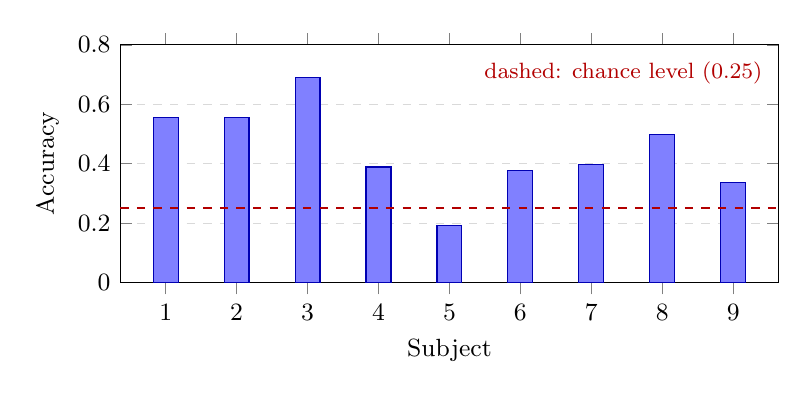
\begin{tikzpicture}
\begin{axis}[
  ybar, bar width=9pt, width=0.82\textwidth, height=4.6cm,
  ymin=0, ymax=0.8, ylabel={Accuracy}, xlabel={Subject}, xtick=data,
  symbolic x coords={1,2,3,4,5,6,7,8,9},
  ymajorgrids, grid style={dashed,gray!30}, enlarge x limits=0.08,
  tick label style={font=\small}, label style={font=\small}]
\addplot[fill=blue!50,draw=blue!70!black] coordinates
  {(1,0.556)(2,0.556)(3,0.691)(4,0.389)(5,0.191)(6,0.378)(7,0.396)(8,0.497)(9,0.337)};
\draw[red!70!black,thick,dashed] (rel axis cs:0,0.3125) -- (rel axis cs:1,0.3125);
\node[anchor=north east,font=\footnotesize,text=red!70!black] at (rel axis cs:0.99,0.97) {dashed: chance level (0.25)};
\end{axis}
\end{tikzpicture}
\caption{Per-subject accuracy on the unseen session.}
\label{fig:acc}
\end{figure}

\textbf{Accuracy.} The decoder is correct 44.3\% of the time, so it is wrong on
more than half of all decisions. Performance varies widely between subjects,
from 0.691 (subject~3) down to 0.191 (subject~5, below chance). Subject~5 is
retained on purpose, as a below-chance decoder is the case a shared-control
law must handle. Because the classes are balanced, $\kappa = (\text{acc}-0.25)/0.75$
exactly, so $\kappa$ is reported only for comparison with the literature.

\textbf{Comparison with published results.} Mean $\kappa$ (0.258) is below the
value of about 0.4 commonly reported for this dataset. Data leakage was ruled
out: for subjects 4 and 9 the held-out session scores higher than
within-session cross-validation, which leakage would not produce. Subject~3
reaches $\kappa = 0.784$ under cross-validation, confirming that the pipeline
works. The gap reflects signal drift between recording days. Higher published
figures typically rely on within-session evaluation or filter-bank CSP.

\textbf{Calibration.} Platt scaling reduced the mean ECE from 0.196 to 0.096 and
improved every subject. The calibrated confidence is informative but weak.
Across all 2592 test trials it averages 0.514 on correct decisions and 0.408 on
incorrect ones (ROC AUC 0.676), and within individual subjects the separation is
smaller.

\textbf{Latency.} Subjects 1, 3 and 7 typically become confident within the
first window (median 2.0\,s). For subjects 4, 5, 6 and 9, 83--100\% of trials
never reach the threshold within 4\,s. Some subjects show a bimodal
distribution, so latency will be resampled empirically in Stage~2 rather than
fitted to a parametric form.

\textbf{Baseline carried forward.} The decoder is now frozen. Stage~2 receives,
for every test trial, the correctness of the decision, the per-subject confusion
matrix, the calibrated confidence and the decision latency. Together these
define the error rate, error direction, confidence term and loop delay of the
simulated BCI channel.

\section{Remaining Work (Stage 2)}

\begin{enumerate}
  \item Fit a per-subject Markov error model and latency distribution from the Stage~1 outputs.
  \item Implement the wheelchair and double-integrator plants and the delayed-PD operator.
  \item Implement the LQR and Dynamic Window Approach controllers.
  \item Implement fixed, confidence-only and risk-gated adaptive arbitration, $\alpha = c(1-r)$.
  \item Derive $\tau_{\max}(\alpha)$ and $\alpha^*$ analytically and verify them numerically.
  \item Compare all policies over 9 subjects, 3 environments and 20 seeds on success rate, collision rate and retained user authority.
  \item Consolidate results, ablations and limitations in the final report.
\end{enumerate}

\section{Limitations of Stage 1}

The EEG is recorded offline and cannot respond to the wheelchair's motion, so it
enters the loop only through measured statistics. The cued, randomised protocol
may produce different error patterns from a self-paced BCI. Latency is estimated
from sliding windows and is heavily censored for some subjects. Finally, the
decoder is standard rather than state of the art, by design.

\section{Note}

This project is under active development. Stage~1 is complete and documented
here. Stage~2 is in the development phase, and the source code will be uploaded
to the repository after the mid-semester evaluation.

\begin{thebibliography}{9}\small
\bibitem{bci} C. Brunner et al., \emph{BCI Competition 2008 -- Graz data set A}, Graz University of Technology, 2008.
\bibitem{moabb} V. Jayaram and A. Barachant, ``MOABB: trustworthy algorithm benchmarking for BCIs,'' \emph{J. Neural Eng.}, 15(6), 2018.
\bibitem{mne} A. Gramfort et al., ``MEG and EEG data analysis with MNE-Python,'' \emph{Front. Neurosci.}, 7:267, 2013.
\bibitem{pf} G. Pfurtscheller and C. Neuper, ``Motor imagery and direct brain--computer communication,'' \emph{Proc. IEEE}, 89(7), 2001.
\bibitem{csp} H. Ramoser, J. M\"uller-Gerking and G. Pfurtscheller, ``Optimal spatial filtering of single trial EEG during imagined hand movement,'' \emph{IEEE Trans. Rehabil. Eng.}, 8(4), 2000.
\bibitem{platt} J. C. Platt, ``Probabilistic outputs for support vector machines,'' in \emph{Advances in Large Margin Classifiers}, MIT Press, 1999.
\bibitem{dragan} A. D. Dragan and S. S. Srinivasa, ``A policy-blending formalism for shared control,'' \emph{Int. J. Robot. Res.}, 32(7), 2013.
\bibitem{dwa} D. Fox, W. Burgard and S. Thrun, ``The dynamic window approach to collision avoidance,'' \emph{IEEE Robot. Autom. Mag.}, 4(1), 1997.
\end{thebibliography}

\end{document}
